\documentclass[11pt]{article}
\usepackage[margin=1in]{geometry}
\usepackage{amsmath,amssymb,array,booktabs,graphicx,longtable}
\usepackage[hidelinks]{hyperref}
\usepackage{url}
\newcommand{\citep}[1]{\cite{#1}}
\makeatletter
\renewcommand{\@cite}[2]{(#1\if@tempswa, #2\fi)}
\makeatother
\newcommand{\PaperTitle}{Fixed Heavy-Tailed Probabilistic Forecasting under Missing Historical Observations}
\newcommand{\ShortTitle}{Heavy-Tailed Forecasts with Missingness}
\newcommand{\StudentT}{Student-$t$}
\newcommand{\df}{\mathrm{df}}

\setlength{\parindent}{1.2em}
\setlength{\parskip}{0.25em}
\setlength{\emergencystretch}{4em}
\graphicspath{{figures/}}

\begin{document}
\title{\PaperTitle}
\author{\textbf{[AUTHOR INPUT REQUIRED]}\\
\small Affiliations: [AUTHOR INPUT REQUIRED]\\
\small Corresponding author and email: [AUTHOR INPUT REQUIRED]\\
\small ORCID identifiers: [AUTHOR INPUT REQUIRED]}
\date{}
\maketitle
\begin{center}
\small Running title: \ShortTitle
\end{center}

\begin{abstract}
Forecasting systems often require predictive uncertainty as well as point forecasts, yet incomplete historical observations change the error distribution used to estimate that uncertainty. Comparisons are additionally weakened when competing methods see different missingness realizations. We study probabilistic time-series forecasting under fixed masks applied only to historical inputs, with train-only normalization and paired evaluation assets. A lightweight distribution head represents each horizon--channel marginal with a fixed Student-$t$ distribution with degrees of freedom $8$, using the same trainable location and scale projections as Gaussian and Laplace alternatives. Proper probabilistic scores are central: negative log-likelihood and a Monte Carlo estimate of the continuous ranked probability score are reported alongside point-prediction noninferiority. On fixed TimePerceiver checkpoints, Student-$t$ improves negative log-likelihood in 12/12 dataset--seed pairs and is noninferior for both continuous ranked probability score and point prediction in 12/12. A distribution-head ablation supports fixed heavy tails over learned degrees of freedom in the evaluated protocol. On PatchTST, probabilistic-score gains appear in 3/3 datasets, while Electricity exceeds the prespecified point-error tolerance. The results support fixed heavy-tailed predictive distributions as a lightweight method for improving probabilistic forecast quality under missing historical observations, while the PatchTST Electricity result cautions against assuming metric-wise invariance across backbones.

\end{abstract}
\noindent\textbf{Keywords:} probabilistic forecasting; time-series forecasting; missing observations; Student-$t$ distribution; proper scoring rules; heavy-tailed errors

\section{Introduction}
\label{sec:introduction}

Forecasting decisions require more than a point estimate when the costs of under- and over-prediction differ. Predictive distributions express uncertainty across the forecast horizon and support decisions that depend on tail risk, quantiles, or intervals. Modern probabilistic forecasting therefore evaluates the entire distribution, not only its center \citep{gneiting2007proper,gneiting2014probabilistic,salinas2020deepar}.

Historical observations are often incomplete. Missing values can remove recent evidence, entire channels, or contiguous blocks, changing both point errors and the residual shape available to a probability model. Recurrent imputation methods, deep generative imputers, and masked forecasting architectures address different parts of this problem \citep{cao2018brits,che2018grud,fortuin2020gpvae,tashiro2021csdi,du2023saits,lee2025timeperceiver}, but Gaussian residual assumptions can remain fragile when errors become heavy-tailed.

Probabilistic forecasts should be compared with proper scores that reward honest distributions. Negative log-likelihood (NLL) is distribution-sensitive, while the continuous ranked probability score (CRPS) evaluates calibration and sharpness together \citep{matheson1976crps,gneiting2007proper,jordan2019scoringrules}. Mean squared error (MSE) and mean absolute error (MAE) remain useful point criteria, but neither replaces distributional evaluation. Coverage and width are likewise diagnostics rather than complete quality measures in isolation.

Paired comparisons also require identical evaluation inputs. If Gaussian and heavy-tailed heads are evaluated under independently sampled masks, mask variation can be mistaken for a distribution-head effect. We therefore fix train, validation, and test splits; fit normalization on training data only; and reuse the same validation and test masks within every comparison.

The proposed final specification is deliberately small: a fixed \StudentT{} predictive marginal with $\df=8$. Gaussian, Laplace, and fixed \StudentT{} variants have identical trainable location and scale projections; the fixed head adds no trainable degrees-of-freedom parameter. The value $8$ is a reference setting that is empirically sufficient in the distribution-head ablation, not a theoretically optimal or dataset-specific choice.

The evidence combines missing-history degradation, four probability-head seeds on fixed TimePerceiver checkpoints, a distribution-family ablation, a PatchTST replication, efficiency measurements, and retained negative results. Our contributions are: (i) a fixed-mask protocol for paired probabilistic forecasting under missing historical observations; (ii) controlled evidence that a matched-capacity fixed heavy-tailed head improves proper scores on the evaluated TimePerceiver conditions; and (iii) a transparent second-backbone assessment showing that probabilistic-score gains transfer while a small Electricity point-error tradeoff prevents a complete multi-metric conclusion.

\section{Related Work}
\label{sec:related-work}

\subsection{Probabilistic forecasting and proper scores}
DeepAR established autoregressive probabilistic forecasting at scale \citep{salinas2020deepar}; spline quantile functions and diffusion-based TimeGrad broadened the available forecast distributions \citep{gasthaus2019spline,rasul2021timegrad}. Proper-score methodology distinguishes distributional quality from point accuracy \citep{matheson1976crps,gneiting2007proper,gneiting2007calibration,gneiting2014probabilistic}. We report NLL and a sampled CRPS implementation, with interval scores and coverage--width diagnostics as complementary summaries \citep{winkler1972interval,jordan2019scoringrules}.

\subsection{Heavy-tailed predictive distributions}
The Student distribution originates from small-sample inference \citep{student1908} and has long been used for robust modeling because heavier tails reduce the penalty assigned to extreme residuals relative to a Gaussian model \citep{lange1989robust}. Our use is narrower: we replace only the marginal forecast likelihood while keeping trainable location and scale capacity matched. The work neither introduces a new distribution nor learns a separate tail parameter for the final method.

\subsection{Forecasting with incomplete histories}
GRU-D, BRITS, GP-VAE, CSDI, and SAITS represent influential approaches to irregular or missing time-series data \citep{che2018grud,cao2018brits,fortuin2020gpvae,tashiro2021csdi,du2023saits}. TimePerceiver directly motivates the backbone and missing-history setting studied here \citep{lee2025timeperceiver}. Our focus differs from imputation-only evaluation: future targets remain intact, and the forecast distribution is scored after fixed historical masking.

\subsection{Forecasting backbones, calibration, and comparison}
Informer, Autoformer, FEDformer, the Temporal Fusion Transformer, and PatchTST illustrate diverse sequence-modeling choices for long-horizon forecasting \citep{zhou2021informer,wu2021autoformer,zhou2022fedformer,lim2021tft,nie2023patchtst}. Post-hoc probabilistic calibration and conformal intervals offer complementary tools \citep{kuleshov2018calibrated,romano2019cqr,stankeviciute2021conformal}, although dependent time series require careful temporal splits. Finally, paired forecast comparisons should separate descriptive consistency from formal inferential testing \citep{diebold1995comparison,giacomini2006conditional}; the present study reports no formal significance test.

\section{Forecasting Problem}
\label{sec:forecasting-problem}

Let $x_{1:t}\in\mathbb{R}^{t\times C}$ denote a $C$-channel historical series observed up to forecast origin $t$, and let $y_{t+1:t+H}$ be the future target over horizon $H$. A binary historical observation mask $m_{1:t}$ marks available values. The model receives the masked historical input $\widetilde{x}_{1:t}$ together with the time covariates required by the backbone. Only historical inputs are masked; future targets are never masked or exposed to the model.

For every horizon $h$ and channel $c$, the probabilistic head estimates a predictive marginal distribution
\begin{equation}
p(y_{t+h,c}\mid\widetilde{x}_{1:t},m_{1:t}).
\label{eq:marginal-forecast}
\end{equation}
The point forecast is the predicted location. Central marginal prediction intervals are obtained from the corresponding distribution quantiles. These are horizon--channel marginals: the method does not estimate a joint covariance structure, a multivariate predictive density, or joint coverage.

The official chronological train, validation, and test splits are retained. Normalization statistics are fitted on training data only and reused for validation and test. Fixed mask assets define random, block, channel, and mixed missingness at rates $0.1$, $0.3$, $0.5$, and $0.7$ for the deterministic audit. Probability-head comparisons use paired fixed masks, preventing mask resampling from confounding distribution-family differences.

\section{Probabilistic Forecasting Method}
\label{sec:method}

\subsection{Matched-capacity marginal heads}
Given a frozen backbone representation $z_{h,c}$, two linear projections produce location $\mu_{h,c}$ and a positive scale $\sigma_{h,c}=\operatorname{softplus}(s_{h,c})+\epsilon$. Gaussian, Laplace, and fixed \StudentT{} heads use exactly these trainable projections. The fixed head is
\begin{equation}
y_{t+h,c}\sim \operatorname{StudentT}(\df=8,\mu_{h,c},\sigma_{h,c}).
\label{eq:student-head}
\end{equation}
Thus it adds no trainable degrees-of-freedom parameters. A learned-$\df$ version is included only as an ablation and is not the proposed final method.

The fixed value $\df=8$ is a reference degrees-of-freedom setting. It is empirically sufficient under the evaluated distribution-head protocol, not theoretically optimal, and was not selected separately for each dataset. One goal of the ablation is to ask whether extra tail flexibility is supported once location and scale capacity are controlled.

\subsection{Training objective and forecast summaries}
Probability heads minimize validation-selected NLL while the official backbone checkpoint remains fixed. No test observation or target is used for head selection. NLL is a distribution-sensitive proper score. CRPS is another proper score that combines calibration and sharpness; here it is estimated with 64 Monte Carlo samples using the fixed evaluation seed 52025, rather than reported as an exact analytic value. MSE and MAE evaluate the location forecast.

For marginal intervals, prediction interval coverage probability (PICP) and mean prediction interval width (MPIW) describe coverage and sharpness separately. Neither PICP alone nor width alone is sufficient. The interval score combines coverage penalties with width for each marginal interval \citep{winkler1972interval}. These diagnostics do not imply joint calibration.

\section{Evaluation Design}
\label{sec:evaluation}

\subsection{Datasets and fixed missing-history protocol}
Experiments use ETTh1, Weather, and Electricity with input length 384 and prediction length 96. The official splits and preprocessing rules are preserved, normalization is fitted on training data only, and fixed validation and test masks are reused within paired comparisons. Historical inputs alone are masked. The test set is never used for training, hyperparameter selection, early stopping, or conformal calibration.

The deterministic audit covers four mask types and four rates. The probabilistic TimePerceiver and PatchTST comparisons use the corrected fixed-mask pipeline; invalid historical runs in which masks were not applied are excluded from every result. Head selection uses validation NLL. Gaussian and \StudentT{} heads within a pair use the same backbone checkpoint, mask, split, target, training budget, and evaluation code.

\subsection{Seed scope and decision criteria}
The TimePerceiver comparison uses four probability-head training seeds (2021, 2022, 2023, and 2025) on a fixed official backbone checkpoint per dataset. It is therefore a probability-head seed study, not an end-to-end backbone retraining study. The PatchTST comparison uses one backbone seed and one probability-head seed (2025) per dataset under random missingness at rate $0.3$.

The paired criteria require lower NLL, CRPS noninferiority, and point-prediction noninferiority. Point noninferiority permits a relative MSE increase of at most $1\%$:
\begin{equation}
\frac{\operatorname{MSE}_{t}-\operatorname{MSE}_{g}}{\operatorname{MSE}_{g}}\leq 0.01,
\label{eq:point-gate}
\end{equation}
where subscripts $t$ and $g$ denote fixed \StudentT{} and Gaussian heads. This tolerance was fixed before the second-backbone decision. Test results do not alter it. All reported comparisons are descriptive; no formal significance test is performed.

\section{Empirical Results}
\label{sec:results}

\subsection{Forecast degradation under missing history}
Across 48 dataset--mask--rate cells, deterministic error rises as more historical values are removed. Table~\ref{tab:fixed-mask-degradation} gives the representative matrix and Figure~\ref{fig:missingness-degradation} shows the complete rate trends; full tables appear in the supplement.

\begin{table}[t]
\centering
\caption{Deterministic forecast degradation under fixed historical masks. MSE is lower-is-better; relative degradation uses the corresponding clean TimePerceiver forecast as reference.}
\label{tab:fixed-mask-degradation}
\scriptsize
\resizebox{\linewidth}{!}{\begin{tabular}{@{}lrrrr@{}}
\toprule
Dataset & Mask & Rate & MSE & Clean degradation \\
\midrule
ETTh1 & Block & 0.30 & 0.423837 & 13.19\% \\
ETTh1 & Channel & 0.30 & 0.583704 & 55.88\% \\
ETTh1 & Mixed & 0.30 & 0.495055 & 32.20\% \\
ETTh1 & Random & 0.10 & 0.378811 & 1.16\% \\
ETTh1 & Random & 0.30 & 0.425394 & 13.60\% \\
ETTh1 & Random & 0.50 & 0.525856 & 40.43\% \\
Electricity & Block & 0.30 & 0.184630 & 47.28\% \\
Electricity & Channel & 0.30 & 0.391038 & 211.92\% \\
Electricity & Mixed & 0.30 & 0.246785 & 96.86\% \\
Electricity & Random & 0.10 & 0.138429 & 10.42\% \\
Electricity & Random & 0.30 & 0.200572 & 59.99\% \\
Electricity & Random & 0.50 & 0.325732 & 159.83\% \\
Weather & Block & 0.30 & 0.180420 & 25.24\% \\
Weather & Channel & 0.30 & 0.284471 & 97.47\% \\
Weather & Mixed & 0.30 & 0.224939 & 56.14\% \\
Weather & Random & 0.10 & 0.169631 & 17.75\% \\
Weather & Random & 0.30 & 0.240810 & 67.16\% \\
Weather & Random & 0.50 & 0.331313 & 129.99\% \\
\bottomrule
\end{tabular}
}
\end{table}

\begin{figure}[t]
\centering
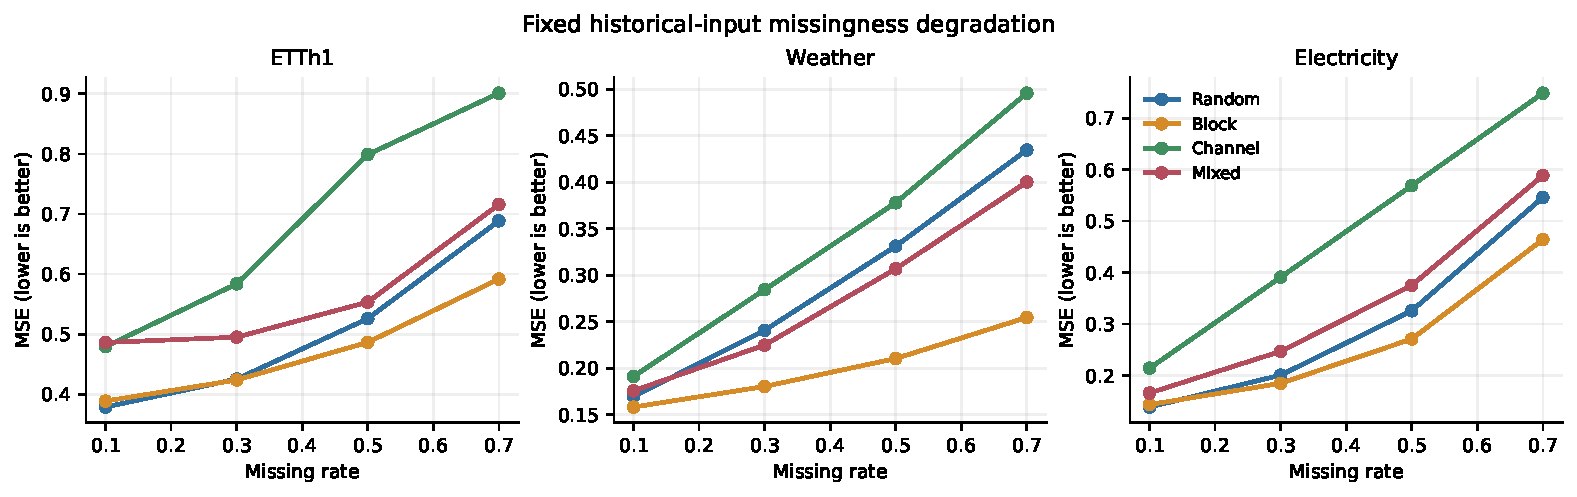
\includegraphics[width=0.96\linewidth]{fig1_missingness_degradation.pdf}
\caption{MSE under fixed historical-mask assets. Line styles and markers distinguish mask types in addition to color, and larger missing rates generally increase forecast error.}
\label{fig:missingness-degradation}
\end{figure}

\subsection{TimePerceiver paired proper-score results}
Across 12 dataset--seed pairs, the \StudentT{} variant improves NLL in 12/12 cases, is CRPS-noninferior in 12/12 cases, and satisfies point noninferiority in 12/12 cases. These are four probability-head seeds on a fixed backbone checkpoint for each dataset. Table~\ref{tab:timeperceiver-multiseed} reports dataset means and variability; Figure~\ref{fig:timeperceiver-nll} retains every paired NLL delta.

\begin{table}[t]
\centering
\caption{TimePerceiver results across four probability-head seeds on fixed backbone checkpoints. Deltas are fixed \StudentT{} minus Gaussian; negative NLL and CRPS deltas indicate improvement.}
\label{tab:timeperceiver-multiseed}
\scriptsize
\resizebox{\linewidth}{!}{\begin{tabular}{@{}lrrrrrrrrrrr@{}}
\toprule
Dataset & G NLL & T NLL & $\Delta$NLL & NLL wins & G CRPS & T CRPS & $\Delta$CRPS & G MSE & T MSE & $\Delta$MSE & Point NI \\
\midrule
ETTh1 & 0.915014 & 0.871113 & -0.043900 & 4 & 0.342011 & 0.337656 & -0.004356 & 0.416862 & 0.415611 & -0.001252 & 4 \\
Weather & 0.577226 & 0.103670 & -0.473557 & 4 & 0.244788 & 0.207544 & -0.037245 & 0.210306 & 0.209818 & -0.000488 & 4 \\
Electricity & 0.439644 & 0.365348 & -0.074296 & 4 & 0.209365 & 0.207395 & -0.001970 & 0.167419 & 0.167703 & 0.000284 & 4 \\
\bottomrule
\end{tabular}
}
\end{table}

\begin{figure}[t]
\centering
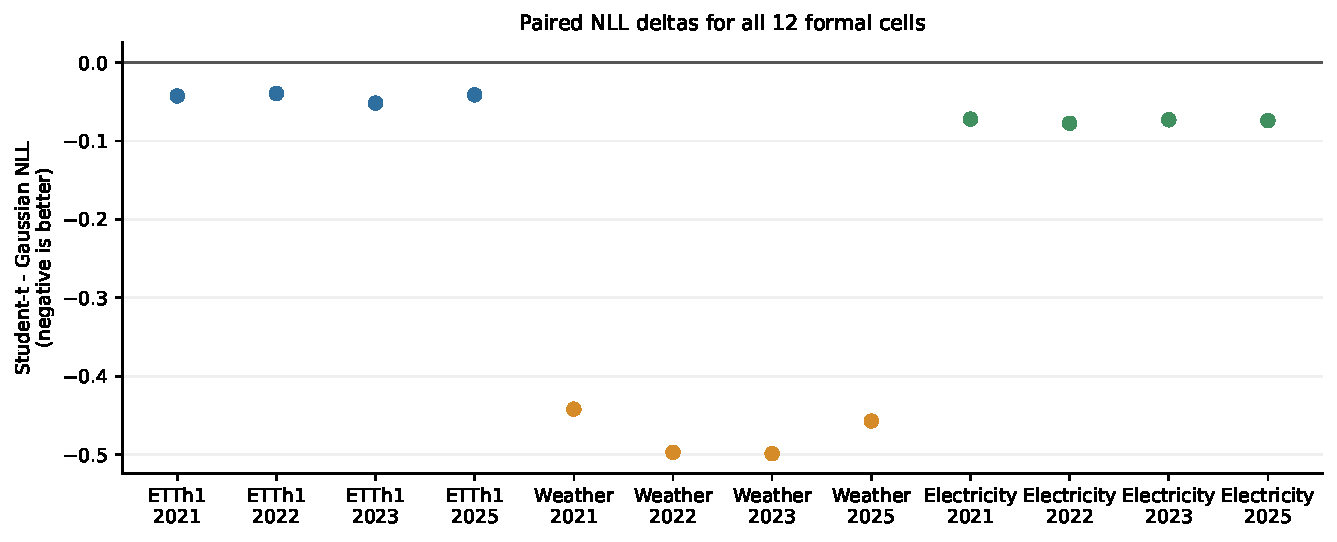
\includegraphics[width=0.96\linewidth]{fig2_multiseed_nll_deltas.pdf}
\caption{Paired TimePerceiver NLL deltas for all dataset--head-seed pairs. Negative values favor the fixed \StudentT{} forecast distribution.}
\label{fig:timeperceiver-nll}
\end{figure}

\subsection{Distribution-family ablation}
The matched-head ablation compares Gaussian, Laplace, fixed \StudentT{}, and learned-$\df$ \StudentT{} forecasts. Table~\ref{tab:distribution-ablation} and Figure~\ref{fig:distribution-ablation} support fixed heavy-tailed forecasting rather than learned degrees of freedom. Fixed $\df=8$ is sufficient under the evaluated protocol, whereas learning per-channel $\df$ provides no consistent additional benefit. The earlier learned-$\df$ results remain visible in the ablation.

\begin{table}[t]
\centering
\caption{Distribution-head ablation on frozen TimePerceiver checkpoints. Gaussian, Laplace, and fixed \StudentT{} share identical trainable location and scale capacity; lower NLL, CRPS, MSE, and MAE are better.}
\label{tab:distribution-ablation}
\scriptsize
\resizebox{\linewidth}{!}{\begin{tabular}{@{}lrrrrrr@{}}
\toprule
Dataset & Head & NLL & CRPS & MSE & Coverage error & Trainable \\
\midrule
etth1 & Gaussian & 0.918535 & 0.344127 & 0.420332 & 0.038132 & 6,168 \\
etth1 & Laplace & 0.879116 & 0.341785 & 0.424149 & 0.011910 & 6,168 \\
etth1 & Fixed Student-t (df=8) & 0.864949 & 0.336548 & 0.413927 & 0.022006 & 6,168 \\
etth1 & Learned Student-t & 0.877154 & 0.340263 & 0.419177 & 0.020301 & 6,175 \\
weather & Gaussian & 0.586325 & 0.245442 & 0.212237 & 0.082667 & 24,624 \\
weather & Laplace & 0.204399 & 0.209589 & 0.210051 & 0.070806 & 24,624 \\
weather & Fixed Student-t (df=8) & 0.136165 & 0.208461 & 0.210994 & 0.051632 & 24,624 \\
weather & Learned Student-t & 0.129293 & 0.208276 & 0.210836 & 0.052156 & 24,645 \\
electricity & Gaussian & 0.440598 & 0.209453 & 0.167881 & 0.038304 & 24,624 \\
electricity & Laplace & 0.370388 & 0.208768 & 0.170436 & 0.018222 & 24,624 \\
electricity & Fixed Student-t (df=8) & 0.367009 & 0.207797 & 0.168473 & 0.018744 & 24,624 \\
electricity & Learned Student-t & 0.366449 & 0.207786 & 0.168486 & 0.018502 & 24,945 \\
\bottomrule
\end{tabular}
}
\end{table}

\begin{figure}[t]
\centering
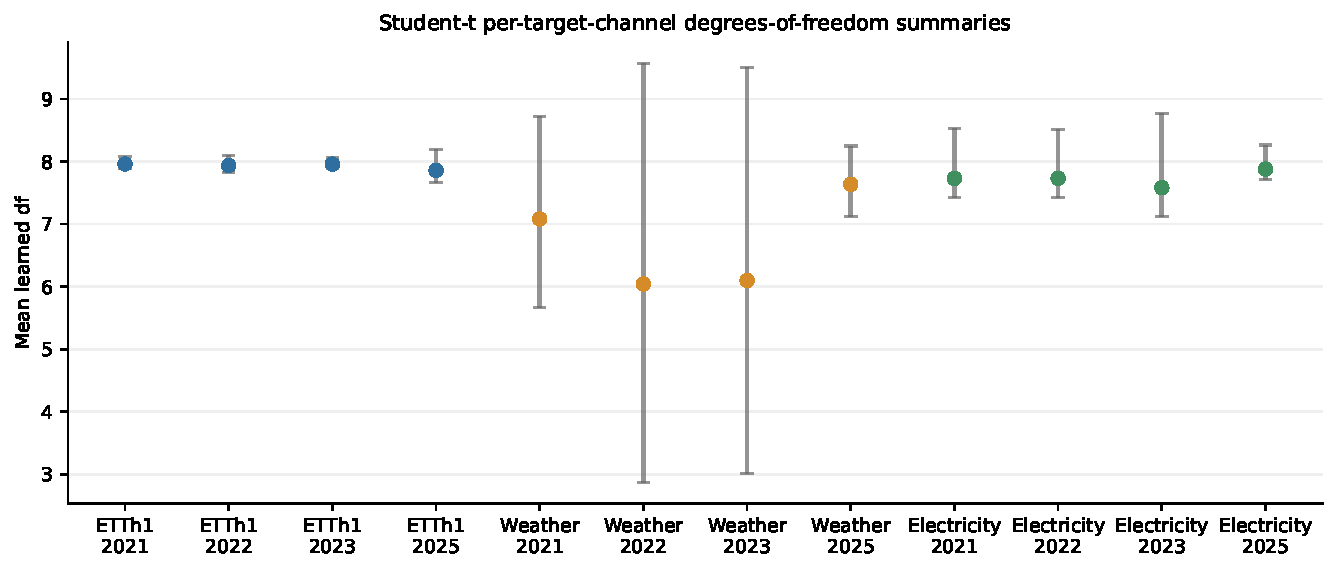
\includegraphics[width=0.88\linewidth]{fig4_student_t_df.pdf}
\caption{Distribution-head comparison under random historical missingness at rate $0.3$. The fixed $\df=8$ setting is a common reference value, not a dataset-specific selection.}
\label{fig:distribution-ablation}
\end{figure}

\subsection{PatchTST replication and point tradeoff}
PatchTST records NLL wins in 3/3 datasets, CRPS noninferiority in 3/3, point noninferiority in 2/3, and a full paired pass in 2/3. ETTh1 and Weather pass all paired criteria. For Electricity, Gaussian MSE is 0.165829 and fixed \StudentT{} MSE is 0.167809, a change of +0.001980 or +1.194\%. This exceeds the prespecified 1\% point-noninferiority threshold. Thus probabilistic-score gains transfer to the second evaluated backbone, but complete multi-metric consistency does not.

\begin{table}[t]
\centering
\caption{PatchTST fixed \StudentT{} minus Gaussian deltas. Negative NLL and CRPS values indicate improvement. Electricity's +1.194\% relative MSE change exceeds the 1\% point-noninferiority threshold.}
\label{tab:patchtst}
\scriptsize
\resizebox{\linewidth}{!}{\begin{tabular}{@{}lrrrrrrrrr@{}}
\toprule
Dataset & Backbone & $\Delta$NLL & $\Delta$CRPS & $\Delta$MSE & Rel. MSE & NLL win & CRPS NI & Point NI & Full pair \\
\midrule
ETTh1 & TimePerceiver & -0.053587 & -0.007578 & -0.006405 & -1.524\% & Yes & Yes & Yes & Yes \\
ETTh1 & PatchTST & -0.035317 & -0.002538 & -0.005439 & -1.274\% & Yes & Yes & Yes & Yes \\
Weather & TimePerceiver & -0.450160 & -0.036981 & -0.001243 & -0.586\% & Yes & Yes & Yes & Yes \\
Weather & PatchTST & -1.818698 & -0.076205 & -0.050179 & -21.595\% & Yes & Yes & Yes & Yes \\
Electricity & TimePerceiver & -0.073589 & -0.001656 & 0.000592 & +0.353\% & Yes & Yes & Yes & Yes \\
Electricity & PatchTST & -0.083433 & -0.001688 & 0.001980 & +1.194\% & Yes & Yes & No & No \\
\bottomrule
\end{tabular}
}
\end{table}

\begin{figure}[t]
\centering
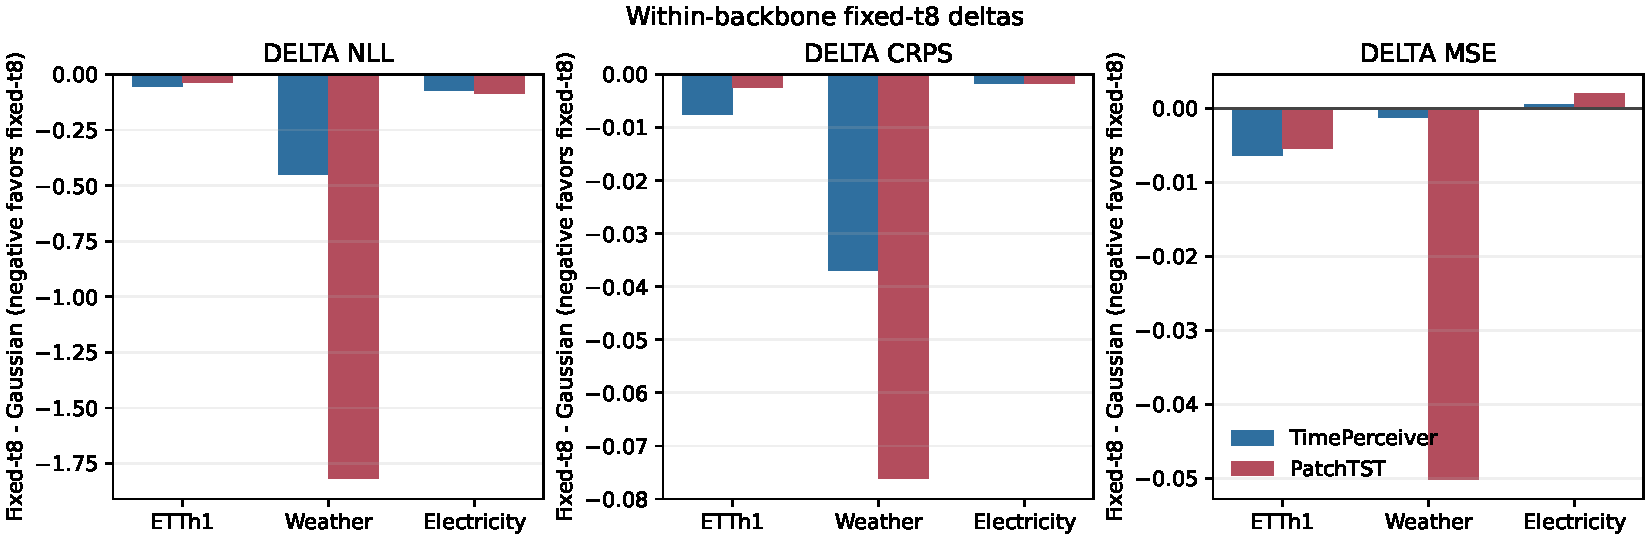
\includegraphics[width=0.96\linewidth]{fig_gate5b_cross_backbone_deltas.pdf}
\caption{Within-backbone metric deltas for TimePerceiver and PatchTST. Negative values favor fixed \StudentT{}; the positive PatchTST Electricity MSE delta is retained.}
\label{fig:cross-backbone}
\end{figure}

\subsection{Efficiency}
Fixed \StudentT{} has the same number of trainable head parameters as Gaussian and Laplace because $\df$ is not learned. Table~\ref{tab:efficiency} reports controlled timing and memory measurements. Comparisons are interpreted within each benchmark environment, not as hardware-independent throughput claims.

\begin{table}[t]
\centering
\caption{Controlled probability-head parameter, runtime, and memory measurements. Values are compared within dataset and benchmark environment.}
\label{tab:efficiency}
\scriptsize
\resizebox{\linewidth}{!}{\begin{tabular}{@{}lrrrrrr@{}}
\toprule
Dataset & Head & Params & Forward ms & NLL ms & CRPS ms & Peak MiB \\
\midrule
etth1 & Gaussian & 6,168 & 29.997997 & 51.514500 & 86.934799 & 215.033691 \\
etth1 & Laplace & 6,168 & 29.996887 & 30.016349 & 63.189127 & 215.033691 \\
etth1 & Fixed Student-t (df=8) & 6,168 & 29.902914 & 65.900001 & 90.256716 & 215.034180 \\
etth1 & Learned Student-t & 6,175 & 29.982518 & 69.371223 & 103.335362 & 215.034180 \\
weather & Gaussian & 24,624 & 59.357760 & 79.919755 & 188.685383 & 630.664551 \\
weather & Laplace & 24,624 & 58.485584 & 59.293318 & 133.341993 & 630.664551 \\
weather & Fixed Student-t (df=8) & 24,624 & 58.181018 & 98.037041 & 211.123562 & 630.665039 \\
weather & Learned Student-t & 24,645 & 59.026097 & 97.896011 & 212.516092 & 630.665039 \\
electricity & Gaussian & 24,624 & 356.894562 & 359.007118 & 1248.479182 & 4626.902832 \\
electricity & Laplace & 24,624 & 345.290164 & 343.346301 & 895.849843 & 4626.902832 \\
electricity & Fixed Student-t (df=8) & 24,624 & 343.877731 & 374.742924 & 1477.667372 & 4626.904297 \\
electricity & Learned Student-t & 24,945 & 420.384170 & 473.496327 & 1890.070674 & 4626.904297 \\
\bottomrule
\end{tabular}
}
\end{table}

\subsection{Tail-concentrated gains}
Residual-percentile decompositions place much of the NLL improvement in the most extreme Gaussian-residual bins. Figure~\ref{fig:tail-gains} presents both evaluated backbones. These diagnostics are descriptive and do not establish a causal mechanism or treat forecast elements as independent inferential samples.

\begin{figure}[t]
\centering
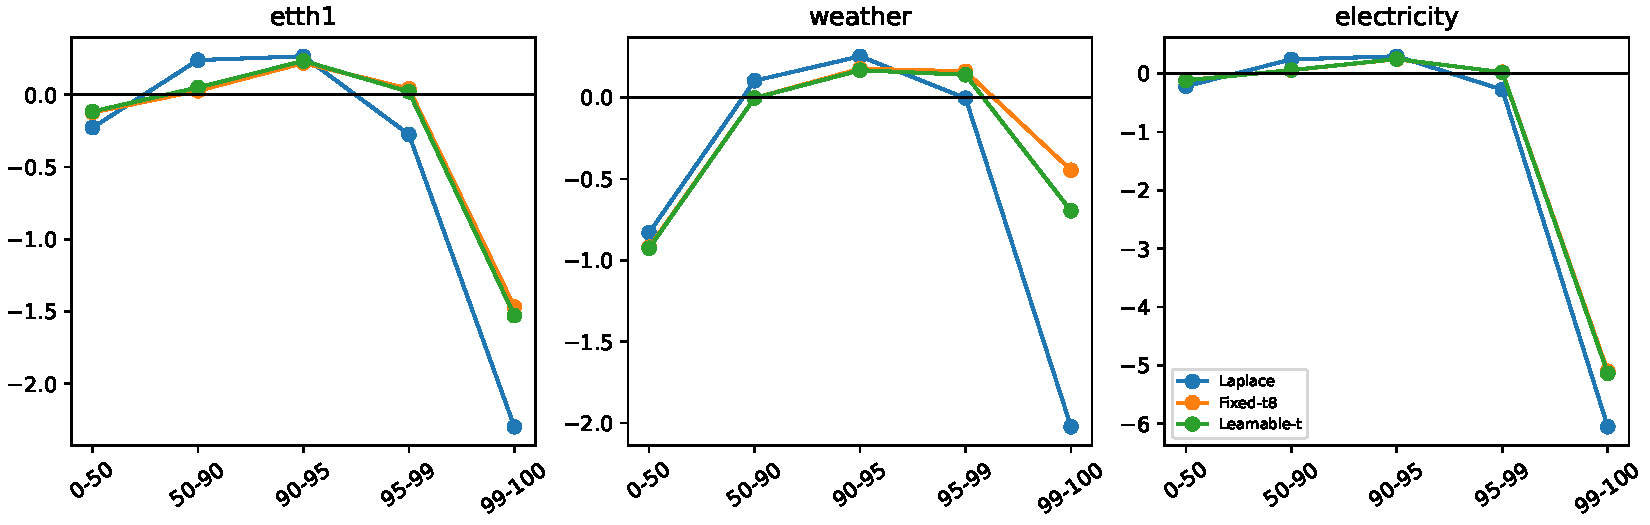
\includegraphics[width=0.48\linewidth]{fig_gate5a_tail_nll_gain.pdf}
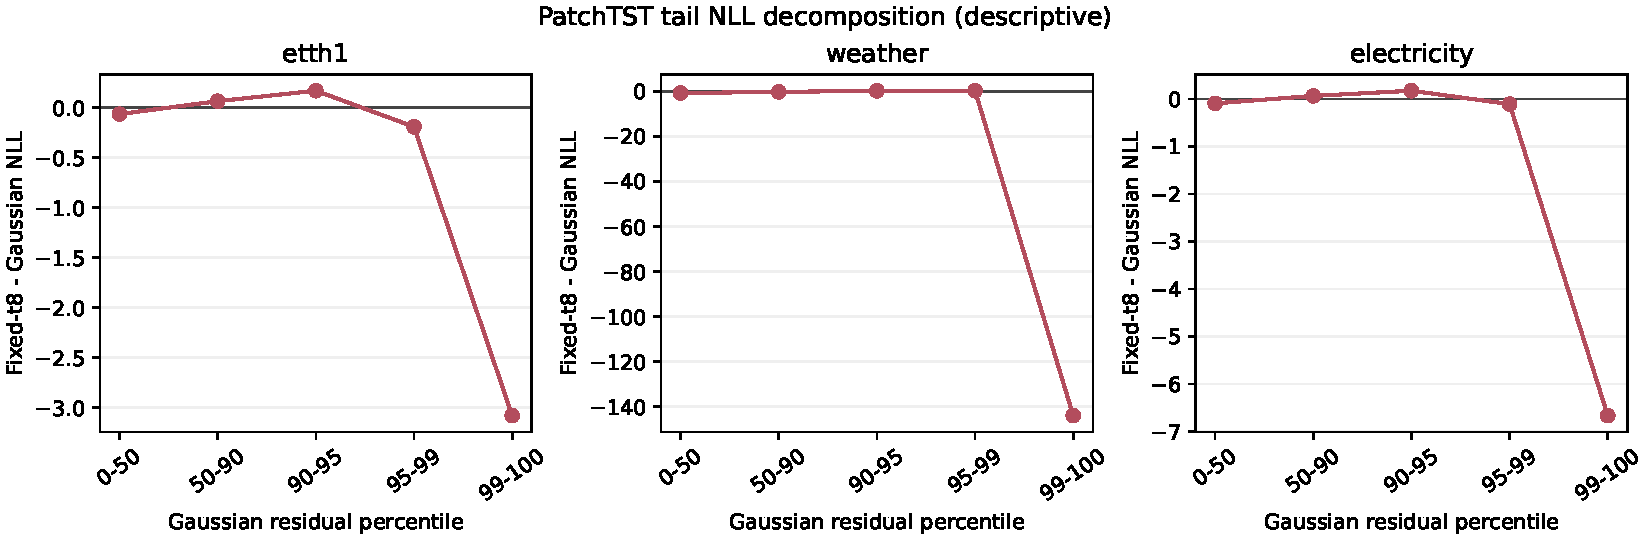
\includegraphics[width=0.48\linewidth]{fig_gate5b_patchtst_tail_nll_gain.pdf}
\caption{Descriptive NLL differences across Gaussian-residual percentile bins for TimePerceiver (left) and PatchTST (right). Negative values favor fixed \StudentT{}.}
\label{fig:tail-gains}
\end{figure}

\section{Diagnostics and Negative Results}
\label{sec:negative-results}

The retained negative results constrain the interpretation. On ETTh1 with random missingness at rate $0.3$, a matched-capacity static adapter improves the official forecast, but the tested missingness-aware FiLM adapter does not improve over that static adapter. Mechanism checks show nonconstant conditioning, nonzero FiLM modulation, finite gradients, and parameter updates. The result therefore concerns this global-statistics conditioning design and fixed condition; it does not establish that missingness conditioning is generally unhelpful.

Under a strict raw-time selection and calibration split, the evaluated additive split-conformal correction widens intervals without improving absolute coverage error. Native intervals are already near the nominal targets, while the calibration segment is descriptively harder. This is a result for one additive score, split, dataset, and missingness condition; it does not generalize to other conformal designs. Detailed tables and figures for both negative findings are in the supplement.

\section{Discussion}
\label{sec:discussion}

\subsection{Why heavy tails help}
The residual-bin analyses show that NLL gains are concentrated in extreme Gaussian-residual regions on both evaluated backbones. This pattern is consistent with a heavier-tailed forecast assigning less implausibly small density to large errors. It is descriptive, not causal proof: the experiments do not manipulate tail behavior independently of the likelihood family.

\subsection{Why a fixed degree of freedom can suffice}
A fixed $\df$ provides robust tails without adding learned shape parameters. One possible explanation for the learned-$\df$ result is that per-channel flexibility may add estimation variance or be weakly identified under the available head-training data. This remains a hypothesis. The evidence only shows that learned $\df$ did not yield a consistent additional gain in this ablation.

\subsection{Proper-score versus point tradeoff}
The PatchTST Electricity case illustrates why distributional and point objectives must be reported together. Better NLL and CRPS can coexist with a small MSE deterioration because the proper scores evaluate the predictive distribution while MSE evaluates its center. The +1.194\% deterioration exceeds the fixed 1\% tolerance, so it is a genuine protocol-level tradeoff rather than a rounding artifact.

\subsection{Practical interpretation}
The supported use case is a forecasting system that requires marginal predictive uncertainty under incomplete historical inputs and can retain paired fixed-mask evaluation. Fixed \StudentT{} is attractive here because it changes the likelihood without increasing trainable head capacity. This interpretation does not imply a particular business deployment, joint uncertainty, or invariant point performance across architectures.

\section{Limitations}
\label{sec:limitations}

The evidence covers three datasets and two backbones with fixed historical masks. Some conditions are single-seed. TimePerceiver varies four probability-head seeds while holding the backbone checkpoint fixed, and PatchTST uses one backbone seed and one head seed under random missingness at rate $0.3$ only. PatchTST Electricity has a point-prediction tradeoff. No formal significance test is reported.

The predictive distributions are marginal by horizon and channel. We do not model joint covariance, assess joint coverage, or report a multivariate energy score. The fixed $\df=8$ value is not theoretically optimal, and the study does not perform dataset-specific tail selection. The conformal study covers a limited additive split procedure, and the FiLM study covers a limited global conditioning design.

The experiments do not evaluate decision-specific economic loss, domain-specific forecast value, density forecast combination, or operational consequences. These are untested extensions rather than implied benefits. Broader missingness shifts, more independently trained backbones, and alternative tail models are needed before stronger generalization claims are warranted.

\section{Conclusion}
\label{sec:conclusion}

This study evaluates a matched-capacity fixed \StudentT{} forecast head under fixed masks applied only to historical observations. Proper probabilistic scores improve consistently across the evaluated TimePerceiver probability-head seeds, and a distribution ablation supports fixed heavy tails over learned degrees of freedom in this setting. PatchTST reproduces the NLL and CRPS direction on all three datasets but retains a small Electricity MSE tradeoff that exceeds the prespecified tolerance. The resulting conclusion is deliberately bounded: fixed heavy-tailed predictive marginals are a lightweight way to improve probabilistic forecast quality under the evaluated missing-history protocol, but point behavior and broader generalization must be checked for each backbone and condition.


\section*{Statements and Declarations}
\textbf{Data availability.} The datasets are publicly available from their original repositories; sources and preprocessing details are documented in the supplementary material.\\
\textbf{Code availability.} [AUTHOR ACTION REQUIRED: provide the verified repository URL and release timing.]\\
\textbf{Funding, conflicts, and contributions.} [AUTHOR INPUT REQUIRED.]\\
\textbf{Generative AI.} [AUTHOR CONFIRMATION REQUIRED: see the separate disclosure draft.]

\begin{thebibliography}{99}

\bibitem[Lee and Lee, 2025]{lee2025timeperceiver} Lee, Jaebin; Lee, Hankook (2025). TimePerceiver: An Encoder-Decoder Framework for Generalized Time-Series Forecasting. \emph{Advances in Neural Information Processing Systems}, vol. 38. \url{https://proceedings.neurips.cc/paper_files/paper/2025/hash/c6c682ba9bd8839104f2a82901da4109-Abstract-Conference.html}.

\bibitem[Nie et al., 2023]{nie2023patchtst} Nie, Yuqi; Nguyen, Nam H.; Sinthong, Phanwadee; Kalagnanam, Jayant (2023). A Time Series is Worth 64 Words: Long-term Forecasting with Transformers. \emph{International Conference on Learning Representations}. \url{https://openreview.net/forum?id=Jbdc0vTOcol}.

\bibitem[Salinas et al., 2020]{salinas2020deepar} Salinas, David; Flunkert, Valentin; Gasthaus, Jan; Januschowski, Tim (2020). {DeepAR}: Probabilistic Forecasting with Autoregressive Recurrent Networks. \emph{International Journal of Forecasting}, vol. 36, no. 3, pp. 1181--1191. \url{https://doi.org/10.1016/j.ijforecast.2019.07.001}.

\bibitem[Gneiting and Raftery, 2007]{gneiting2007proper} Gneiting, Tilmann; Raftery, Adrian E. (2007). Strictly Proper Scoring Rules, Prediction, and Estimation. \emph{Journal of the American Statistical Association}, vol. 102, no. 477, pp. 359--378. \url{https://doi.org/10.1198/016214506000001437}.

\bibitem[Matheson and Winkler, 1976]{matheson1976crps} Matheson, James E.; Winkler, Robert L. (1976). Scoring Rules for Continuous Probability Distributions. \emph{Management Science}, vol. 22, no. 10, pp. 1087--1096. \url{https://doi.org/10.1287/mnsc.22.10.1087}.

\bibitem[Gneiting et al., 2007]{gneiting2007calibration} Gneiting, Tilmann; Balabdaoui, Fadoua; Raftery, Adrian E. (2007). Probabilistic Forecasts, Calibration and Sharpness. \emph{Journal of the Royal Statistical Society: Series B (Statistical Methodology)}, vol. 69, no. 2, pp. 243--268. \url{https://doi.org/10.1111/j.1467-9868.2007.00587.x}.

\bibitem[Gneiting and Katzfuss, 2014]{gneiting2014probabilistic} Gneiting, Tilmann; Katzfuss, Matthias (2014). Probabilistic Forecasting. \emph{Annual Review of Statistics and Its Application}, vol. 1, pp. 125--151. \url{https://doi.org/10.1146/annurev-statistics-062713-085831}.

\bibitem[Jordan et al., 2019]{jordan2019scoringrules} Jordan, Alexander; Krueger, Fabian; Lerch, Sebastian (2019). Evaluating Probabilistic Forecasts with scoringRules. \emph{Journal of Statistical Software}, vol. 90, no. 12, pp. 1--37. \url{https://doi.org/10.18637/jss.v090.i12}.

\bibitem[Gasthaus et al., 2019]{gasthaus2019spline} Gasthaus, Jan; Benidis, Konstantinos; Wang, Yuyang; Rangapuram, Syama Sundar; Salinas, David; Flunkert, Valentin; Januschowski, Tim (2019). Probabilistic Forecasting with Spline Quantile Function RNNs. \emph{Proceedings of the Twenty-Second International Conference on Artificial Intelligence and Statistics}, vol. 89, pp. 1901--1910. \url{https://proceedings.mlr.press/v89/gasthaus19a.html}.

\bibitem[Rasul et al., 2021]{rasul2021timegrad} Rasul, Kashif; Seward, Calvin; Schuster, Ingmar; Vollgraf, Roland (2021). Autoregressive Denoising Diffusion Models for Multivariate Probabilistic Time Series Forecasting. \emph{Proceedings of the 38th International Conference on Machine Learning}, vol. 139, pp. 8857--8868. \url{https://proceedings.mlr.press/v139/rasul21a.html}.

\bibitem[Student, 1908]{student1908} Student (1908). The Probable Error of a Mean. \emph{Biometrika}, vol. 6, no. 1, pp. 1--25. \url{https://doi.org/10.1093/biomet/6.1.1}.

\bibitem[Lange et al., 1989]{lange1989robust} Lange, Kenneth L.; Little, Roderick J. A.; Taylor, Jeremy M. G. (1989). Robust Statistical Modeling Using the t Distribution. \emph{Journal of the American Statistical Association}, vol. 84, no. 408, pp. 881--896. \url{https://doi.org/10.1080/01621459.1989.10478852}.

\bibitem[Che et al., 2018]{che2018grud} Che, Zhengping; Purushotham, Sanjay; Cho, Kyunghyun; Sontag, David; Liu, Yan (2018). Recurrent Neural Networks for Multivariate Time Series with Missing Values. \emph{Scientific Reports}, vol. 8, pp. 6085. \url{https://doi.org/10.1038/s41598-018-24271-9}.

\bibitem[Cao et al., 2018]{cao2018brits} Cao, Wei; Wang, Dong; Li, Jian; Zhou, Hao; Li, Lei; Li, Yitan (2018). {BRITS}: Bidirectional Recurrent Imputation for Time Series. \emph{Advances in Neural Information Processing Systems}, vol. 31, pp. 6776--6786. \url{https://proceedings.neurips.cc/paper_files/paper/2018/hash/734e6bfcd358e25ac1db0a4241b95651-Abstract.html}.

\bibitem[Fortuin et al., 2020]{fortuin2020gpvae} Fortuin, Vincent; Baranchuk, Dmitry; Raetsch, Gunnar; Mandt, Stephan (2020). {GP-VAE}: Deep Probabilistic Time Series Imputation. \emph{Proceedings of the Twenty Third International Conference on Artificial Intelligence and Statistics}, vol. 108, pp. 1651--1661. \url{https://proceedings.mlr.press/v108/fortuin20a.html}.

\bibitem[Tashiro et al., 2021]{tashiro2021csdi} Tashiro, Yusuke; Song, Jiaming; Song, Yang; Ermon, Stefano (2021). {CSDI}: Conditional Score-based Diffusion Models for Probabilistic Time Series Imputation. \emph{Advances in Neural Information Processing Systems}, vol. 34, pp. 24804--24816. \url{https://proceedings.neurips.cc/paper/2021/hash/cfe8504bda37b575c70ee1a8276f3486-Abstract.html}.

\bibitem[Du et al., 2023]{du2023saits} Du, Wenjie; Cote, David; Liu, Yan (2023). {SAITS}: Self-Attention-based Imputation for Time Series. \emph{Expert Systems with Applications}, vol. 219, pp. 119619. \url{https://doi.org/10.1016/j.eswa.2023.119619}.

\bibitem[Lim et al., 2021]{lim2021tft} Lim, Bryan; Arik, Sercan O.; Loeff, Nicolas; Pfister, Tomas (2021). Temporal Fusion Transformers for Interpretable Multi-horizon Time Series Forecasting. \emph{International Journal of Forecasting}, vol. 37, no. 4, pp. 1748--1764. \url{https://doi.org/10.1016/j.ijforecast.2021.03.012}.

\bibitem[Zhou et al., 2021]{zhou2021informer} Zhou, Haoyi; Zhang, Shanghang; Peng, Jieqi; Zhang, Shuai; Li, Jianxin; Xiong, Hui; Zhang, Wancai (2021). Informer: Beyond Efficient Transformer for Long Sequence Time-Series Forecasting. \emph{Proceedings of the AAAI Conference on Artificial Intelligence}, vol. 35, no. 12, pp. 11106--11115. \url{https://doi.org/10.1609/aaai.v35i12.17325}.

\bibitem[Wu et al., 2021]{wu2021autoformer} Wu, Haixu; Xu, Jiehui; Wang, Jianmin; Long, Mingsheng (2021). Autoformer: Decomposition Transformers with Auto-Correlation for Long-Term Series Forecasting. \emph{Advances in Neural Information Processing Systems}, vol. 34, pp. 22419--22430. \url{https://proceedings.neurips.cc/paper_files/paper/2021/hash/bcc0d400288793e8bdcd7c19a8ac0c2b-Abstract.html}.

\bibitem[Zhou et al., 2022]{zhou2022fedformer} Zhou, Tian; Ma, Ziqing; Wen, Qingsong; Wang, Xue; Sun, Liang; Jin, Rong (2022). {FEDformer}: Frequency Enhanced Decomposed Transformer for Long-term Series Forecasting. \emph{Proceedings of the 39th International Conference on Machine Learning}, vol. 162, pp. 27268--27286. \url{https://proceedings.mlr.press/v162/zhou22g.html}.

\bibitem[Kuleshov et al., 2018]{kuleshov2018calibrated} Kuleshov, Volodymyr; Fenner, Nathan; Ermon, Stefano (2018). Accurate Uncertainties for Deep Learning Using Calibrated Regression. \emph{Proceedings of the 35th International Conference on Machine Learning}, vol. 80, pp. 2796--2804. \url{https://proceedings.mlr.press/v80/kuleshov18a.html}.

\bibitem[Romano et al., 2019]{romano2019cqr} Romano, Yaniv; Patterson, Evan; Candes, Emmanuel J. (2019). Conformalized Quantile Regression. \emph{Advances in Neural Information Processing Systems}, vol. 32, pp. 3538--3548. \url{https://proceedings.neurips.cc/paper_files/paper/2019/hash/5103c3584b063c431bd1268e9b5e76fb-Abstract.html}.

\bibitem[Stankeviciute et al., 2021]{stankeviciute2021conformal} Stankeviciute, Kamile; Alaa, Ahmed M.; van der Schaar, Mihaela (2021). Conformal Time-Series Forecasting. \emph{Advances in Neural Information Processing Systems}, vol. 34. \url{https://proceedings.neurips.cc/paper/2021/hash/312f1ba2a72318edaaa995a67835fad5-Abstract.html}.

\bibitem[Diebold and Mariano, 1995]{diebold1995comparison} Diebold, Francis X.; Mariano, Roberto S. (1995). Comparing Predictive Accuracy. \emph{Journal of Business and Economic Statistics}, vol. 13, no. 3, pp. 253--263. \url{https://doi.org/10.1080/07350015.1995.10524599}.

\bibitem[Giacomini and White, 2006]{giacomini2006conditional} Giacomini, Raffaella; White, Halbert (2006). Tests of Conditional Predictive Ability. \emph{Econometrica}, vol. 74, no. 6, pp. 1545--1578. \url{https://doi.org/10.1111/j.1468-0262.2006.00718.x}.

\bibitem[Winkler, 1972]{winkler1972interval} Winkler, Robert L. (1972). A Decision-Theoretic Approach to Interval Estimation. \emph{Journal of the American Statistical Association}, vol. 67, no. 337, pp. 187--191. \url{https://doi.org/10.1080/01621459.1972.10481224}.

\end{thebibliography}

\end{document}
